% Reference (supervisor's Methodology section title), inert. His paper
% names this section "Methodology" and opens with a one-paragraph roadmap
% naming its own subsections by roman numeral before the first \subsection.
\section{Methodology}
\label{sec:method}

\subsection{Corpora}

DAIGT V2~\cite{Thedrcat2023daigtv2} contains 44,868 argumentative student essays, 27,371 human-written and 17,497 machine-generated by a mixture of 2023-era systems including GPT-3.5, Llama-2, Mistral-7B and Falcon-180B, assembled for a public detection competition~\cite{Kaggle2023llmdetect}. The human side derives from the PERSUADE corpus of student argumentative writing~\cite{Crossley2023persuade}. HC3~\cite{Guo2023close} contains question-answer pairs from five English sources, contrasting human answers with a single generator, GPT-3.5-Turbo-0301, over 85,449 rows~\cite{HelloSimpleAI2023hc3}. The two make a useful pair because they differ in nearly every respect that matters here. DAIGT V2 has many generators, one genre and long documents, HC3 one generator, five source domains and short ones. Both were class-balanced by downsampling the majority class, giving 34,994 and 53,806 rows, which fixes a degenerate single-class predictor at 0.333 weighted F1 rather than something respectable and is what makes the label-free control in Section~\ref{sec:labelfree} readable. Training partitions balance to within 0.002 of parity.

\begin{table}[!ht]
\centering
\caption{Corpus statistics after balancing. Duplication is exact match on lowercased, whitespace-normalised text. Leakage is the share of test documents whose text also appears in training or validation.}
\label{tab:corpora}
\footnotesize
\setlength{\tabcolsep}{3.5pt}
\begin{tabular}{@{}lrr@{}}
\toprule
& DAIGT V2 & HC3 \\
\midrule
Rows, as published & 44,868 & 85,449 \\
Rows, balanced & 34,994 & 53,806 \\
Train / validation / test & 25,196 & 38,785 \\
& 2,800 & 4,289 \\
& 6,998 & 10,732 \\
\midrule
Duplicate rows & 6 (0.01\%) & 6,118 (7.16\%) \\
Duplicate groups & 6 & 5,986 \\
Cross-label duplicate texts & 0 & 0 \\
Collection artefact rows & none found & 483 \\
\midrule
Test leakage, group-aware split & 0 (0.00\%) & 0 (0.00\%) \\
Test leakage, naive stratified & 0 (0.00\%) & 570 (5.30\%) \\
\bottomrule
\end{tabular}
\end{table}

Table~\ref{tab:corpora} gives the duplication audit. DAIGT V2 is essentially free of internal duplication, while HC3 carries 6,118 duplicate rows in 5,986 groups plus 483 collection artefacts, typically stored API failure messages.

\subsection{Partitioning}

That duplication is why the split is group-aware. Documents are grouped by an MD5 hash of their whitespace-normalised, lowercased text and whole groups go to one partition, so no two documents with identical normalised content land on opposite sides of a boundary. The partition is 72/8/20 rather than 80/10/10, since a fifth goes to test first and a tenth of the remainder to validation. Measured directly, the group-aware rule leaks 0 of 10,732 HC3 test documents where a plain stratified split of the same sample leaks 570, or 5.30\%, and DAIGT V2 leaks nothing either way. The split is built once and reused by every model and seed, so comparing two models is never also comparing two evaluation sets.

\subsection{Models and configurations}

Five model families are evaluated. Three are classical, Naive Bayes, logistic regression and a linear support vector machine, each run under bag-of-words and TF-IDF for six classical configurations per dataset. Earlier work at full scale reported only the winning representation per model, so we report the complete grid. Two are transformers, bert-base-uncased~\cite{Devlin2019bert} and microsoft/deberta-v3-base~\cite{He2023debertav3}, fine-tuned with AdamW over a grid of learning rate in $\{2\mathrm{e}{-5}, 3\mathrm{e}{-5}\}$, batch size in $\{16, 32\}$ and weight decay in $\{0.01, 0.1\}$, which is a sixteen-run grid per dataset, eight per model, with the operating point selected on validation weighted F1 and early stopping at patience two.

DeBERTa is the strongest encoder of its size on general language-understanding benchmarks, ahead of both BERT and RoBERTa at comparable parameter counts~\cite{He2023debertav3}, which is reason enough to include it. Two properties matter more for this study specifically. Its disentangled attention separates content from position, the relevant inductive bias when the question is how much of a corpus is separable by form, and its SentencePiece tokeniser~\cite{Kudo2018sentencepiece} encodes leading whitespace whereas BERT's WordPiece does not, which makes the pair a controlled contrast on exactly the cue Section~\ref{sec:tokenisation} examines. Benchmark standing does not by itself predict the outcome here, since the two models are level on DAIGT V2 and separate only on HC3.

Classical models receive lowercased, stopword-filtered, lemmatised text with every non-Latin character removed. Transformers receive raw text, whitespace-normalised only, truncated to 128 tokens. The asymmetry is deliberate, since stripping punctuation and casing removes signal a pretrained transformer can use, but it also confounds any classical-versus-transformer comparison, and Section~\ref{sec:budget} measures that rather than assuming it away.

\subsection{The surface-content decomposition}
\label{sec:decomp-def}

The central instrument of this paper separates how much of a benchmark's human-versus-machine separability is available from surface form alone and how much from content alone. Write $x$ for a document and $y \in \{0, 1\}$ for its label, with $1$ denoting machine-generated. Let $\mathcal{D}_{\text{tr}}$ and $\mathcal{D}_{\text{te}}$ be the fixed training and test partitions. Two maps are defined on the raw text. The surface map $\phi_{\mathrm{S}}$ sends a document to $\mathbb{R}^{47}$, a vector of orthographic statistics described in Section~\ref{sec:features}, and reads no word identity whatsoever. The content map $\phi_{\mathrm{C}}$ first applies the normalisation
\begin{equation}
\label{eq:norm}
\nu(x) = \mathrm{collapse}\Big(\mathrm{map}\big(\mathrm{lower}(x),\, \sigma\big)\Big),
\end{equation}
where $\mathrm{lower}$ lowercases, $\mathrm{map}$ applies the character rule $\sigma$ that keeps a character when it is a lowercase Latin letter or whitespace and replaces it with a space otherwise, and $\mathrm{collapse}$ reduces runs of whitespace to a single space. The normalised text is then sent to raw bag-of-words counts over the training vocabulary. Punctuation, casing and non-ASCII characters cannot survive $\nu$, so they cannot enter the content arm. Word identity never enters $\phi_{\mathrm{S}}$.

Each arm fits one logistic regression on the same training partition,
\begin{equation}
\label{eq:arm}
h_{a}  =  \arg\min_{h} \, \sum_{(x,y) \in \mathcal{D}_{\text{tr}}} \ell\big(h(\phi_{a}(x)), y\big)  +  \tfrac{1}{2C}\lVert h \rVert_2^2 ,
\end{equation}
for $a \in \{\mathrm{S}, \mathrm{C}\}$, with $\ell$ the logistic loss and $C$ fixed at the library default for both arms. Sharing the classifier family and regularisation strength is what makes the two arms comparable, since any difference is then in what the representation carries rather than how it is fitted.

The quantity we report is the error of each arm on the held-out partition,
\begin{equation}
\label{eq:err}
\varepsilon_{a}  =  \frac{1}{|\mathcal{D}_{\text{te}}|}\sum_{(x,y)\in\mathcal{D}_{\text{te}}} \mathbf{1}\big[h_{a}(\phi_{a}(x)) \neq y\big],
\end{equation}
and the separability gap between them,
\begin{equation}
\label{eq:gap}
\Delta  =  \varepsilon_{\mathrm{S}} - \varepsilon_{\mathrm{C}} .
\end{equation}
A gap near zero says orthography alone reaches the same accuracy as content alone on that corpus. A large positive gap says content carries what orthography does not. The surface arm's own error answers a more direct question, how much of the benchmark a detector could pass without reading language at all.

Two properties of $\Delta$ matter. It compares two specific arms rather than partitioning the total separability, since a richer surface featurisation would lower $\varepsilon_{\mathrm{S}}$ and a stronger content model would lower $\varepsilon_{\mathrm{C}}$, so it is a corpus-level comparison under a fixed pair of instruments, and it is not a claim that either corpus is clean. The \emph{full} arm is the fine-tuned transformer on raw text, differing from the other two in model family, parameter count and the amount of text it reads, so we report it as a reference point and draw no conclusion from a transformer-to-classical difference without first matching the text budget.

\begin{figure*}[!t]
\centering
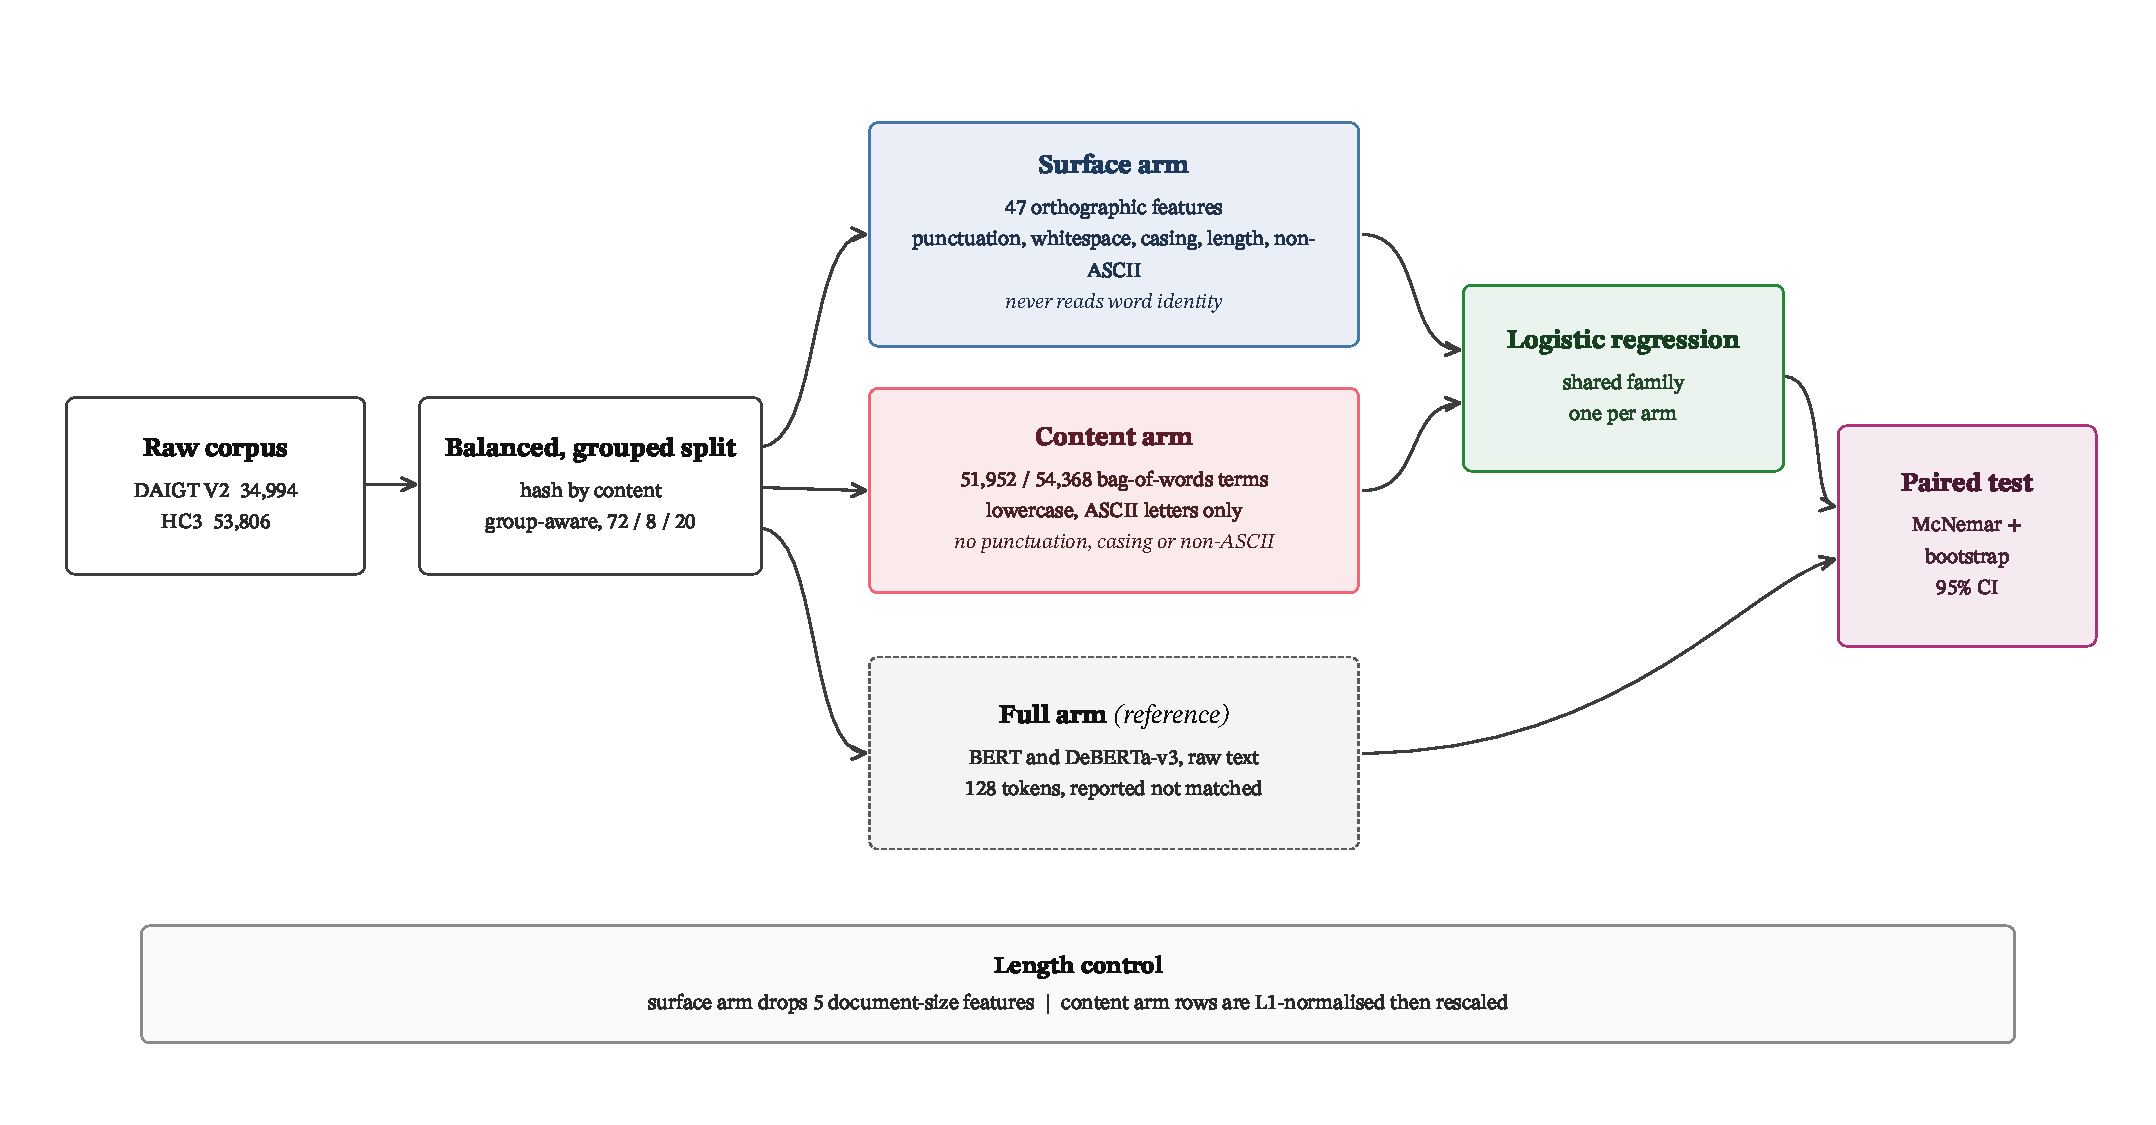
\includegraphics[width=0.82\textwidth]{figures/fig_pipeline.pdf}
\caption{The measurement pipeline. The surface and content arms read disjoint views of every document and share one classifier family. The transformer is a reference, not a matched arm.}
\label{fig:pipeline}
\end{figure*}

Figure~\ref{fig:pipeline} lays out the pipeline end to end, from the balanced, group-aware split through the three arms to the paired significance test each comparison in Section~\ref{sec:results} is drawn from.

\subsection{The length channel and how it is closed}
\label{sec:lengthdef}

One channel survives into both arms, since the surface arm reads character, word and sentence counts directly and raw bag-of-words rows sum to document length, so $\phi_{\mathrm{C}}$ recovers it too. Length is a documented confound on both corpora~\cite{Baidya2026detecting}, so we close it. On the surface side we drop the five features whose magnitude scales with document size, leaving 42 rates and ratios, and write $\phi_{\mathrm{S}}^{-L}$ for the reduced map. Every dropped feature has a rate twin in the same vector, so the cue itself is not removed with the length. On the content side we normalise each row to unit total and rescale by the mean training document length $\bar{n}$,
\begin{equation}
\label{eq:l1}
\phi_{\mathrm{C}}^{-L}(x) = \bar{n} \cdot \frac{\phi_{\mathrm{C}}(x)}{\lVert \phi_{\mathrm{C}}(x) \rVert_1} .
\end{equation}
The rescaling is not cosmetic, since rows summing to one shrink every feature by roughly $\bar{n}$, so at fixed $C$ the effective penalty becomes far heavier and the arm collapses for reasons of scale rather than of length. Section~\ref{sec:length} reports both variants and reads only the rescaled one. We also fit a \emph{length-only} arm on the three pure document-size features, so the shared channel is measured directly rather than inferred from what removing it costs the other two.

\subsection{The surface feature set}
\label{sec:features}

The 47 features cover punctuation-character rates, whitespace behaviour including spaces before punctuation, casing statistics, document and sentence length, non-ASCII and emoji rates, and digit rates. Every one is a count or a rate computable in one pass over the raw string, with no model, no lexicon and no language identification, which is what makes the measurement cheap enough to run on a new corpus before committing to it. Figure~\ref{fig:corr} shows how little they overlap, which matters twice over, since the surface arm's performance is not one cue counted 47 times and the length control removes a small identifiable part of the vector rather than most of it in disguise.

\begin{figure*}[!t]
\centering
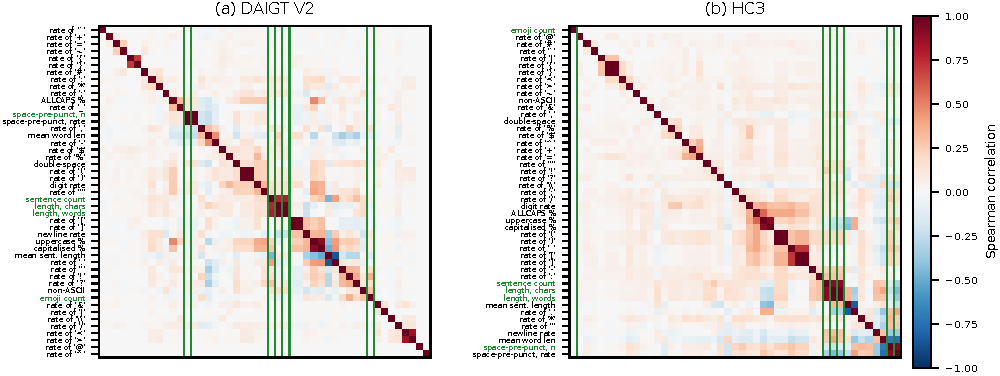
\includegraphics[width=\textwidth]{figures/fig_surface_correlation.pdf}
\caption{Spearman correlation among the 47 surface features on each test split, ordered by average-linkage clustering on $1-|\rho|$ so correlated blocks sit adjacent. The matrix is symmetric, so rows are labelled and columns are not. Features the length control removes are outlined in green. Features with no variance have undefined correlation and are drawn as zero.}
\label{fig:corr}
\end{figure*}

\subsection{Metrics}

We report weighted F1, which is what prior work on these corpora reports, alongside error rate, since F1 compresses at this ceiling and a change from 0.9916 to 0.9972 reads as small while the corresponding error rate falls threefold. For class $c$ with precision $P_c$, recall $R_c$, support $n_c$ and $N=\sum_c n_c$,
\begin{equation}
\label{eq:f1}
\mathrm{F1}_c = \frac{2 P_c R_c}{P_c + R_c}, \quad
\mathrm{F1}_{\mathrm{w}} = \sum_c \frac{n_c}{N}\mathrm{F1}_c, \quad
\mathrm{F1}_{\mathrm{m}} = \frac{1}{|\mathcal{C}|}\sum_c \mathrm{F1}_c .
\end{equation}
Weighted and macro F1 coincide to four decimal places in every row we report, which is the check that no result here is produced by class skew. We also report the area under the ROC curve, since a threshold-free ranking measure can disagree with a thresholded one, and on DAIGT V2 it does.

\subsection{Paired statistics}
\label{sec:stats}

Every transformer baseline is read from the deployed checkpoint's own record rather than from the maximum over its hyperparameter grid, because an earlier version of this analysis compared a grid maximum against a fixed configuration and reported differences that did not exist. Seed spread over three seeds is reported as a range and only for the cell it was measured on, never borrowed across datasets or model families, since fine-tuning outcomes vary materially with initialisation and data order~\cite{Dodge2020fine,Mosbach2020stability}. A range over three runs is not a test statistic, so no comparison here rests on one, and we run no parametric tests at $n \le 30$.

Where two models are compared on the same test set, the comparison is paired, because the two predictions are made on the same documents and treating them as independent samples discards that structure. Let $b$ be the number of documents the first model classifies correctly and the second does not, and $c$ the reverse. Under the null that the two have equal error, the discordant pairs split evenly, so
\begin{equation}
\label{eq:mcnemar}
b \mid (b+c)  \sim  \mathrm{Binomial}\!\left(b+c, \tfrac{1}{2}\right),
\end{equation}
and we report the exact two-sided binomial $p$-value~\cite{McNemar1947note} rather than the chi-squared approximation, which is unreliable when $b+c$ is small, as it is for several comparisons here.

An exact test reports whether a difference is distinguishable from zero, not how large it is, so each comparison also carries a paired bootstrap interval on the error difference~\cite{Efron1979bootstrap}. Writing $e^{(1)}_i$ and $e^{(2)}_i$ for the two models' per-document error indicators, we resample document indices with replacement $B=10{,}000$ times and take the empirical 2.5th and 97.5th percentiles of
\begin{equation}
\label{eq:boot}
\hat{\Delta}^{(b)}  =  \frac{1}{n}\sum_{i \in I_b}\Big(e^{(1)}_i - e^{(2)}_i\Big),
\end{equation}
where $I_b$ is the $b$th resample. Resampling index sets rather than each model's errors independently is what preserves the pairing.

A bootstrap resamples one test set and therefore says nothing about how the corpus was partitioned in the first place. Because the central claim of this paper is a null on HC3, and a null is exactly the kind of claim a single lucky partition can manufacture, the whole decomposition is repeated over five group-aware partitions of the same balanced sample, varying only the split seed. Section~\ref{sec:multisplit} reports what that shows.

\subsection{Controls}
\label{sec:controls}

Three controls guard the claims below, each added after an uncontrolled version of the corresponding experiment produced a conclusion that did not survive. The \emph{pipeline-fires} control exists because our whitespace cleaning produces bit-identical BERT predictions on HC3, which alone is indistinguishable from a cleaning step that never ran, so we apply the same pipeline to DAIGT V2, where it also removes emoji that WordPiece represents, and confirm predictions there do change. The \emph{tokenisation} control compares token identifier sequences for minimally different strings, since whether a detector can exploit a character-level cue is a property of its tokeniser and directly testable. The \emph{label-free} control scores 400 inputs per condition carrying no human-versus-machine information at all, including uniform random character strings, token-shuffled text, punctuation-only strings, a repeated token and the empty string, without which a confident prediction on corrupted input is indistinguishable from a learned response to it.